% gEDA - GPL Electronic Design Automation
% switcap.tex - Switcap symbol library and gnetlist backend documentation
% Copyright (C) 2003 Dan McMahill
%
% This program is free software; you can redistribute it and/or modify
% it under the terms of the GNU General Public License as published by
% the Free Software Foundation; either version 2 of the License, or
% (at your option) any later version.
%
% This program is distributed in the hope that it will be useful,
% but WITHOUT ANY WARRANTY; without even the implied warranty of
% MERCHANTABILITY or FITNESS FOR A PARTICULAR PURPOSE.  See the
% GNU General Public License for more details.
%
% You should have received a copy of the GNU General Public License
% along with this program; if not, write to the Free Software
% Foundation, Inc., 675 Mass Ave, Cambridge, MA 02139, USA.

\documentclass{article}
%\usepackage{epsfig}
\usepackage{graphicx}
% This line will enable hyperlinks in the PDF output
% file.
\usepackage[ps2pdf,breaklinks=true,colorlinks=true]{hyperref}

\setlength{\parindent}{0pt}
\setlength{\parskip}{1ex plus 0.5ex minus 0.2ex}

\title{gEDA/gaf Switcap Symbols and Netlister}
\author{Dan McMahill\\
        \\
        This document is released under GFDL\\ 
	(\url{http://www.gnu.org/copyleft/fdl.html})}
\date{April 13th, 2003}

\begin{document}

\maketitle
\newpage

\tableofcontents
\newpage


\section{Overview}

This document describes the symbol library and gnetlist backend which
supports driving SWITCAP simulations from the gEDA/gaf system.
SWITCAP is a switched capacitor circuit simulator available from
Columbia University.  It is used in many classroom and research
environments.  One drawback to SWITCAP is the lack of a freely
available schematic capture frontend.  The gEDA/gaf SWITCAP symbol
library and gnetlist backend tries to fill that gap.

The basic steps involved with using gEDA as the frontend for SWITCAP
simulations are:

\begin{enumerate}
\item Create schematics of the circuit.
\item Create an analysis file.
\item Extract the netlist.
\item Run the SWITCAP simulation.
\item Run {\tt sw2asc} to extract the results.
\item View the results with {\tt gwave}.
\end{enumerate}

\section{Requirements}
You will need the following programs to be installed.
\begin{enumerate}
\item A recent version of gEDA/gaf.  To see if your version is recent
  enough, see if the directory {\tt \${prefix}/share/gEDA/sym/switcap}
  exists.  {\tt \${prefix}} is the installation prefix for gEDA on
  your system.

\item SWITCAP.  The executable is usually called {\tt sw}.  If you do
  not have SWITCAP available on your system, you will need to contact
  Columbia University to obtain a copy.  The gEDA/gaf SWITCAP support
  was tested with SWITCAP Version A.5R Release 21-Sep-87.

\item Although it is optional, you may wish to install a tool which
  can be used for plotting the output data.  SWITCAP produces both
  ASCII data listings as well as ugly ASCII plots (note the release
  date of the version of SWITCAP used).  Suitable tools are:
  \begin{itemize}
    \item Gwave.  Gwave is an analog waveform viewer.  It is fairly
      basic, but easy to use, includes cursors, and has zoom/pan
      features.  See {\tt http://www.geda.seul.org} 
    \item Scilab.  Similar to matlab.  Powerful, but no cursors or
      panning.  See {\tt http://www-rocq.inria.fr/scilab}
    \item Octave.  Similar to matlab.  See {\tt http://www.octave.org}
    \item Grace.  See {\tt http://plasma-gate.weizmann.ac.il/Grace/}
    \end{itemize}
\end{enumerate}

\section{Creating Schematics}
\subsection{Required Symbols}
This section assumes you are familiar with using gschem to create and
edit schematics.  SWITCAP netlisting is only supported for the
components contained in the SWITCAP symbol library as well as the
ground symbol found in the 'power' library which comes with gEDA.  All
allowed SWITCAP elements except for subcircuits are supported.  You
{\em must} include the following elements on your schematic:

\begin{enumerate}
\item One instance of the switcap-timing symbol.  This symbol will set the
  master clock period for your simulations.
  
\item One or more instances of the switcap-clock symbol.  This symbol
  defines a clock with a particular phase and period.  The reference
  designator of the clock symbol is used by the switches to set what
  phase they switch on.

\item One or more instances of the switcap-analysis symbol.  This symbol
  defines an analysis by specifying a file to include in the SWITCAP
  netlist.  By including multiple instances of this symbol, multiple
  analysis files may be included.

\end{enumerate}

\subsection{Optional Symbols}
You can also optionally add the following SWITCAP special symbols to
your schematic:

\begin{enumerate}
\item Zero or one instance of the switcap-title symbol.  This will add a
  TITLE: line to the SWITCAP netlist and will appear in the output
  file.

\item Zero or one instance of the switcap-options symbol.  By editing the
  OPTIONS attribute on this symbol you can set the various options
  which can be passed to SWITCAP.
\end{enumerate}

\subsection{Net Names}
When creating schematics to drive SWITCAP, you should name all nets
that you wish to plot.  To avoid possible conflicts with unnamed nets,
you should avoid using purely numerical names for nets because
all unnamed nets will be assigned (somewhat randomly) numbers without
checking for possible conflicts with explicitly named nets.
SWITCAP limits the length of node names to 7 characters.

\subsection{Switches}
When placing switches on your schematic, you will need to define
which clock they are controlled with.  This is done by setting
the clock attribute on the switch to the reference designator 
of the clock which should control it.

\section{Extracting the SWITCAP Netlist}
To extract the SWITCAP netlist, run 
\begin{verbatim}
    gnetlist -g switcap -o test.scn file1.sch [file2.sch ...]
\end{verbatim}
For the example file contained in this archive, you can run: 
\begin{verbatim}
    gnetlist -g switcap -o example.scn ckt.sch \ 
        clocks.sch analysis.sch
\end{verbatim}

The netlist will be left in {\tt example.scn}.

\section{Running SWITCAP}
I typically use something like:
\begin{verbatim}
  printf "example.scn\nexample.out\n" | sw
\end{verbatim}
so I can use command history to rerun SWITCAP without having to
manually type the file names each time.

Refer to the SWITCAP manual for more details.

\appendix
\section{Symbols in the Library}

\subsection{Capacitors (switcap-capacitor)}
Ideal capacitor.
Attributes:
\begin{itemize}
\item {\bf C}=capacitance.  Required.  Specifies filename to be
  included.
\item {\bf refdes}=reference designator.  Required.  Must start with
  ``C'' and be unique.
\end{itemize}

\subsection{Switches (switcap-switch)}
Ideal switch.
Attributes:
\begin{itemize}
\item {\bf clock}=Controlling clock.  Required.  Specifies which clock
  controls this switch.
\item {\bf refdes}=reference designator.  Required.  Must start with
  ``S'' and be unique.
\end{itemize}

\subsection{Independent Voltage Sources (switcap-vsrc)}
Attributes:
\begin{itemize}
\item {\bf refdes}=reference designator.  Required.  Must start with
  ``V'' and be unique.
\end{itemize}

\subsection{Dependent Voltage Sources (switcap-vcvs)}
Attributes:
\begin{itemize}
\item {\bf gain}=gain.  Required.  Specifies the gain of the
  controlled source.
\item {\bf refdes}=reference designator.  Required.  Must start with
  ``E'' and be unique.
\end{itemize}

\subsection{Clock Specification (switcap-clock)}
Attributes:
\begin{itemize}
\item {\bf PSTART}=starting clock phase.  Required.  Specifies on what
  phase of the master clock this clock turns on.
\item {\bf PSTOP}=ending clock phase.  Required.  Specifies on what
  phase of the master clock this clock turns off.
\item {\bf PERIOD}=clock period.  Required.  Specifies the period of
  the clock in terms of master clock cycles.
\item {\bf refdes}=reference designator.  Required.  The switches that
  are controlled by this clock will refer to it by the reference
  designator.  As such, avoid running any reference designator
  renumbering tools.
\end{itemize}

\subsection{Master Timing Specification (switcap-timing)}
Attributes:
\begin{itemize}
\item {\bf PERIOD}=clock period.  Required.  Specifies the period of
  the master clock in seconds.
\end{itemize}
Only a single instance of this symbol is allowed.

\subsection{Analysis File Include (switcap-analysis)}
This symbol will cause a specified file containing SWITCAP analysis
commands to be included in the output netlist.
Attributes:
\begin{itemize}
\item {\bf file}=filename.  Required.  Specifies filename to be
  included.
\end{itemize}

\subsection{Simulation Title Specification (switcap-title)}
Attributes:
\begin{itemize}
\item {\bf TITLE}=switcap title.  Required.  Specifies the TITLE
  line for the SWITCAP netlist.
\end{itemize}
Only a single instance of this symbol is allowed.

\subsection{Simulation Options Specification (switcap-options)}
Attributes:
\begin{itemize}
\item {\bf OPTIONS}=switcap options.  Required.  Specifies the OPTIONS
  line for the SWITCAP netlist.  See the SWITCAP manual for allowed
  values. 
\end{itemize}
Only a single instance of this symbol is allowed.


\section{Example}
This appendix provides a simple example of the entire process of
generating a schematic, producing a SWITCAP netlist, running a
simulation, and plotting the results. 

\subsection{Example Schematics}
Figure~\ref{fig:ckt} shows the
schematic of a simple switched capacitor circuit.
\begin{figure}
\begin{center}
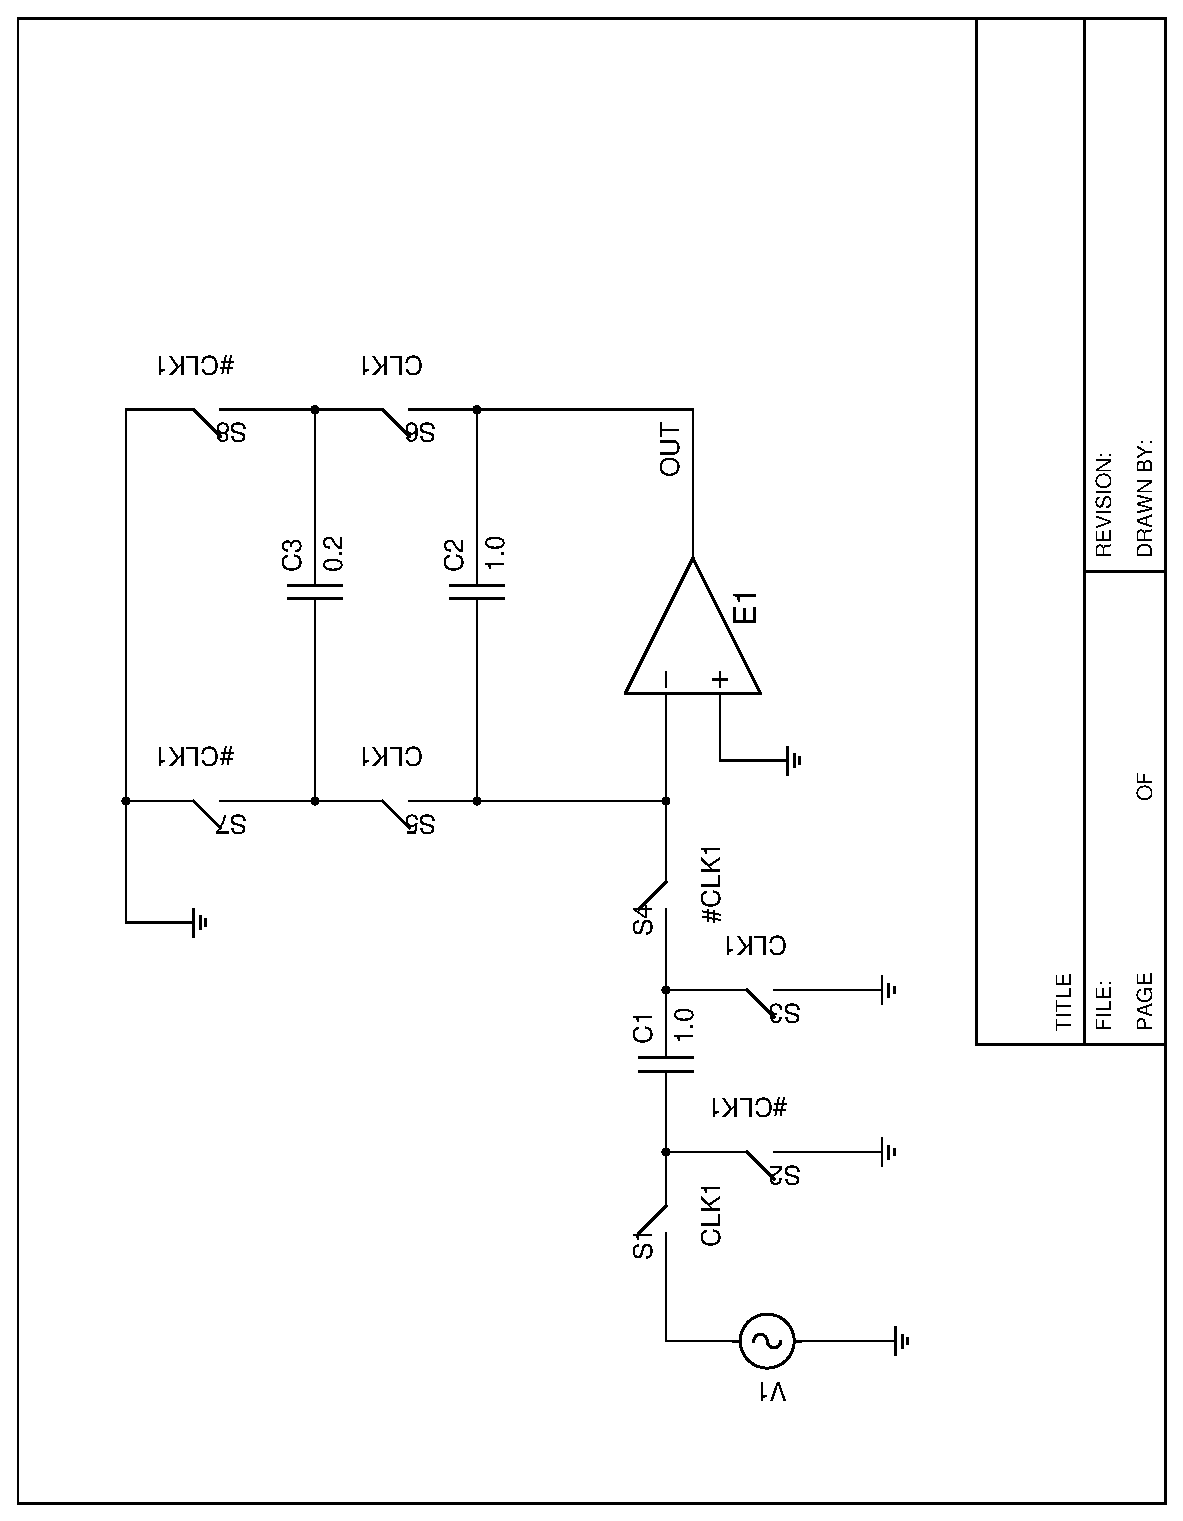
\includegraphics[angle=270,width=4in]{ckt.eps}
\end{center}
\caption{Simple Switched Capacitor Circuit}
\label{fig:ckt}
\end{figure}
Note that some switches, S1 and S3 for example, are controlled by CLK1
while others, S2 and S4 for example, are controlled by the complement
of CLK1 (\#CLK1).  

Figure~\ref{fig:clocks} shows the definition of a clock and the master
clock.  Here we define a master clock period (mcp) of 1.0 $\mu$s in
the timing block.  
\begin{figure}
\begin{center}
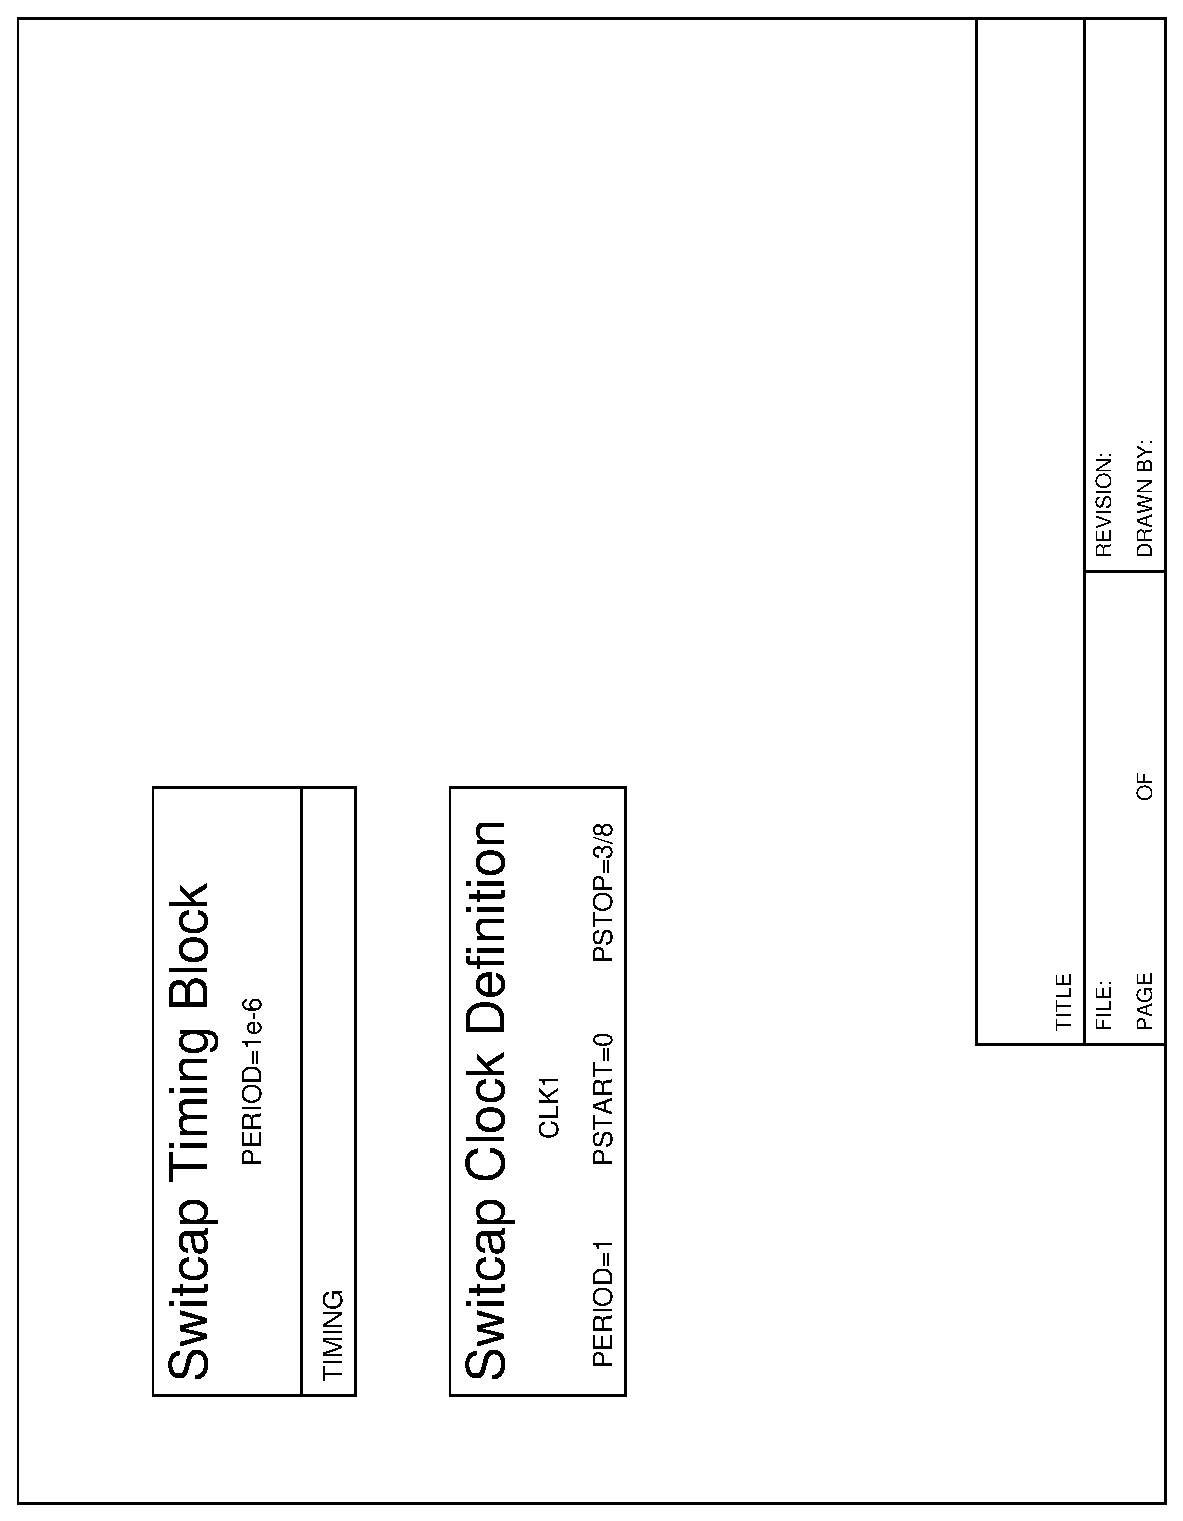
\includegraphics[angle=270,width=4in]{clocks.eps}
\end{center}
\caption{SWITCAP Clock Definition Schematic}
\label{fig:clocks}
\end{figure}
In the clock definition symbol, we define a clock called CLK1 that has
a period equal to 1 master clock period (mcp).  The phase of CLK1
turning on switches is 0 and the phase of CLK1 turning off switches is
3/8 mcp.  Additional clock phases can be defined by creating more
instances of the clock definition symbol.

Figure~\ref{fig:analysis} shows an instantiation of the title block
symbol which will cause ``my title'' to be used in the TITLE line in
the SWITCAP netlist. 
Figure~\ref{fig:analysis} also shows an instantiation of an analysis
block which directs the netlister to include the contents of the file
{\tt test.ana} in the output netlist.  Figure~\ref{fig:test.ana} shows
the contents of the {\tt test.ana} file.
\begin{figure}
\begin{center}
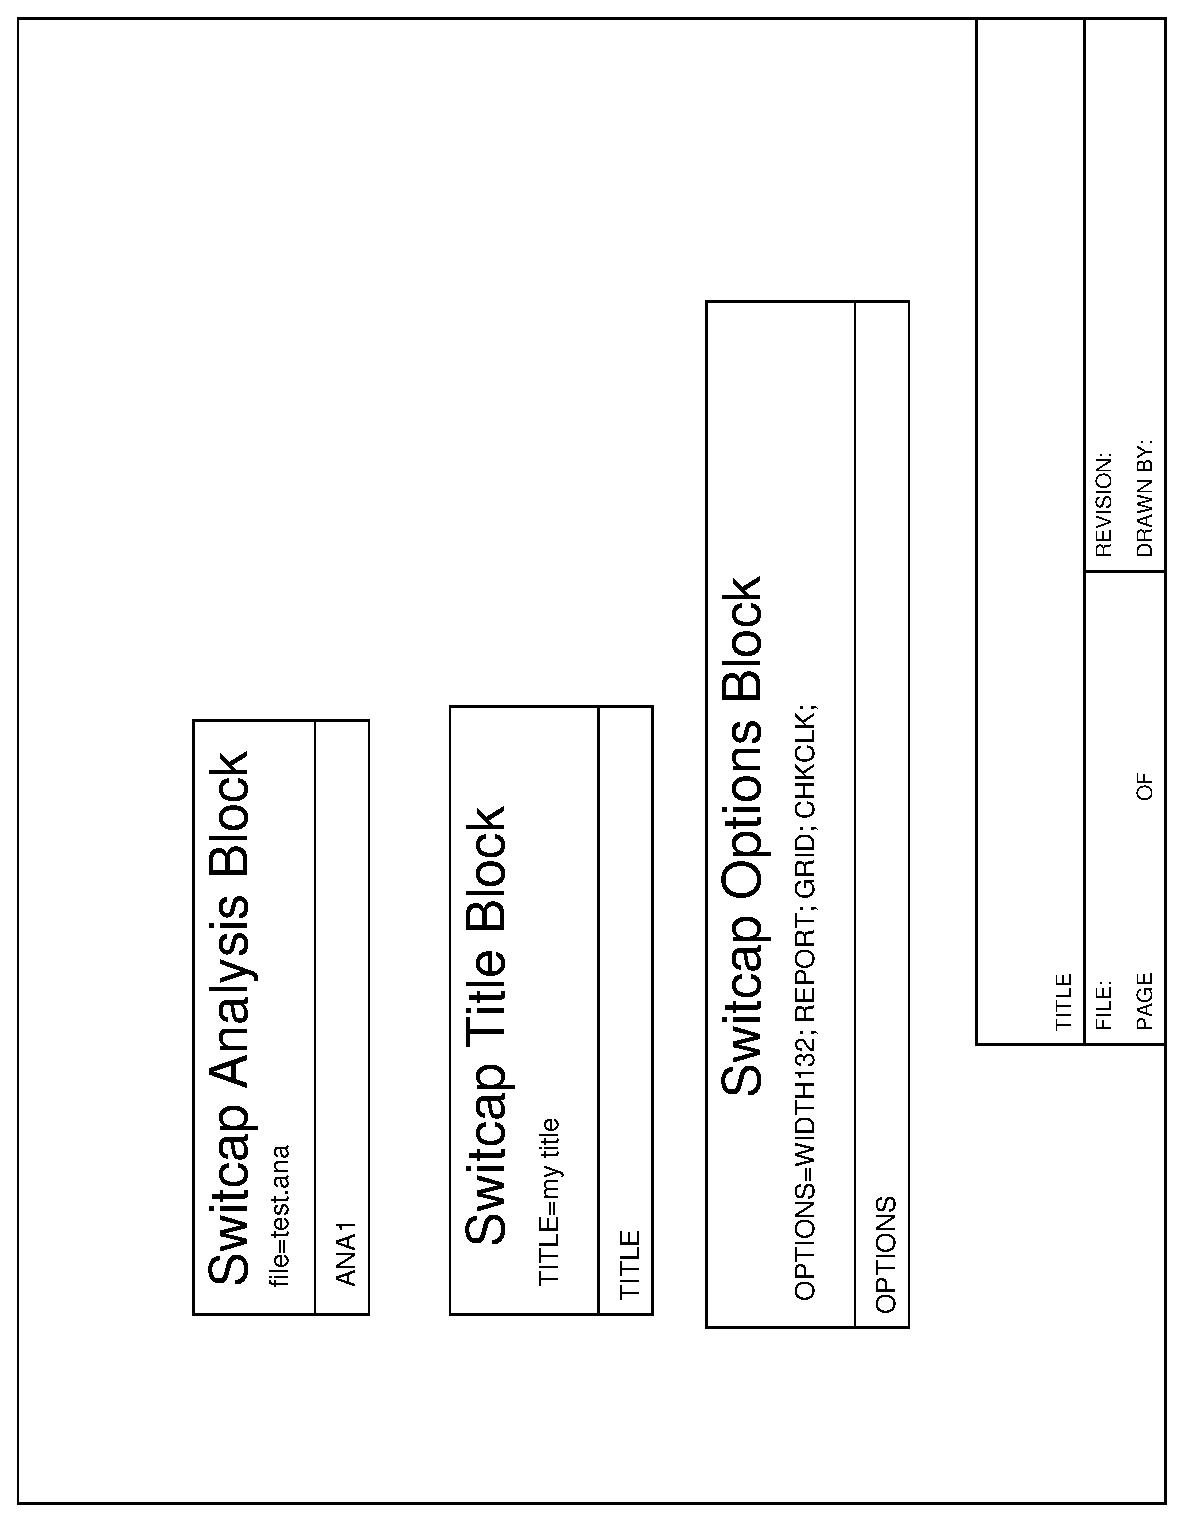
\includegraphics[angle=270,width=4in]{analysis.eps}
\end{center}
\caption{SWITCAP Analysis Definition Schematic}
\label{fig:analysis}
\end{figure}
\begin{figure}
\begin{center}
\begin{verbatim}
ANALYZE SSS;
     INFREQ 100.0 1.0E6 LOG 501;
     SET V1 AC 1.0 0.0;
     PRINT VDB(OUT) VP(OUT);
     END;

ANALYZE TRAN;
     TIME 0+ 500 1
     SET V1 PULSE 0 5 10e-6 5e-6 5e-6 100e-6 500e-6;
     PRINT V(OUT);
     END;
\end{verbatim}
\end{center}
\caption{SWITCAP Analysis File, {\tt test.ana}}
\label{fig:test.ana}
\end{figure}

\subsection{Netlist the Design}
To netlist the design, run:
\begin{verbatim}
    gnetlist -g switcap -o example.scn ckt.sch \ 
        clocks.sch analysis.sch
\end{verbatim}

\subsection{Run the Simulation}
Run the simulation with:
\begin{verbatim}
  printf "example.scn\nexample.out\n" | sw
\end{verbatim}

\subsection{Process the Results}
Convert the SWITCAP output file to something gwave can read by
running:
\begin{verbatim}
  sw2asc example.out
\end{verbatim}

\subsection{Plot the Results}
Start up the {\tt gwave} program and load the first sinusoidal steady
state result by running:
\begin{verbatim}
  gwave example.out.SSS.1.asc
\end{verbatim}
Drag the two waveforms onto the two waveform panels and change the
x-axis to a log scale.  Figure~\ref{fig:gwave_out_sss} shows the output.
\begin{figure}
\begin{center}
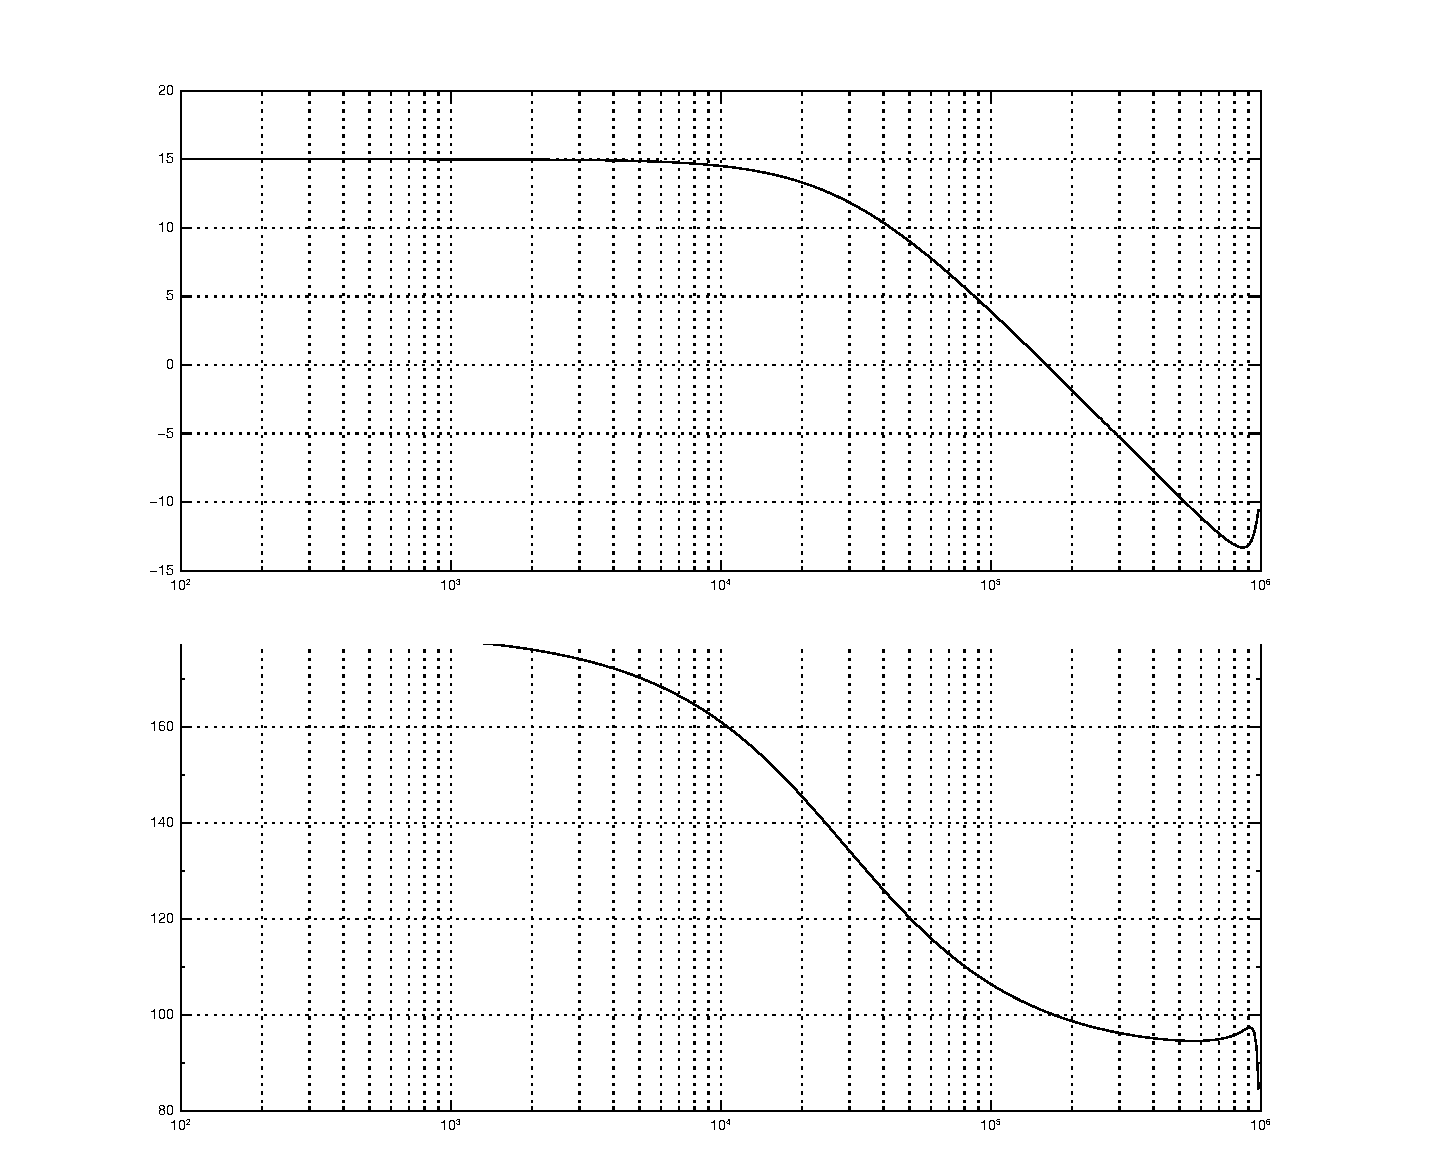
\includegraphics[width=4in]{gwave_out_sss.ps}
\end{center}
\caption{Simulation Results -- Sinusoidal Steady State}
\label{fig:gwave_out_sss}
\end{figure}
Start up the {\tt gwave} program and load the transient
result by running:
\begin{verbatim}
  gwave example.out.TRAN.1.asc
\end{verbatim}
Drag the output waveform onto the waveform panel.
Figure~\ref{fig:gwave_out_tran} shows the output.
\begin{figure}
\begin{center}
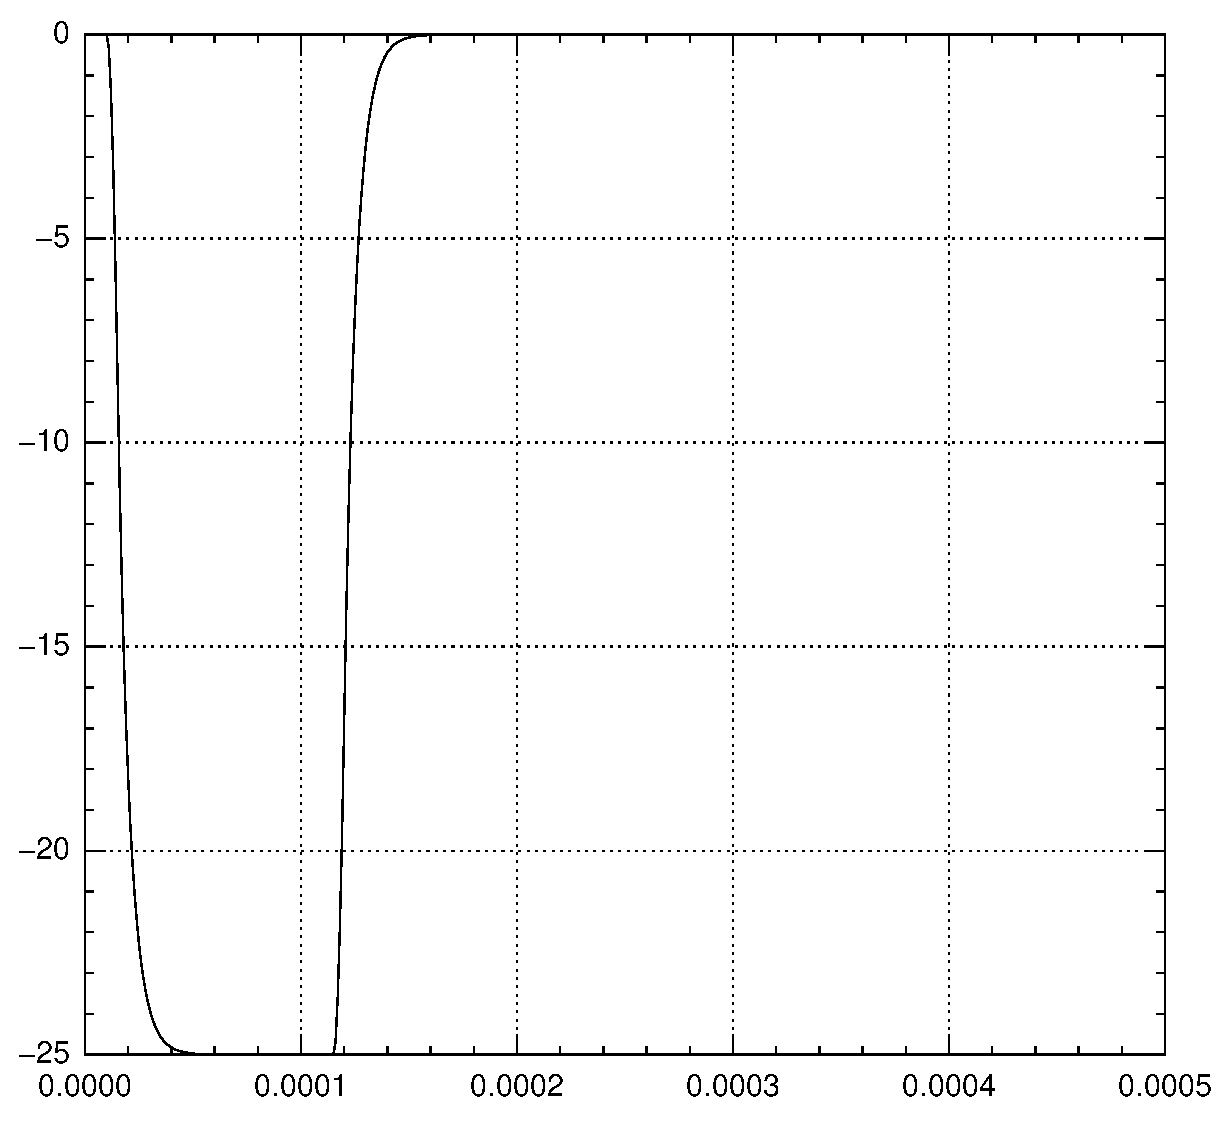
\includegraphics[width=4in]{gwave_out_tran.ps}
\end{center}
\caption{Simulation Results -- Transient}
\label{fig:gwave_out_tran}
\end{figure}

\newpage
\section{Document Revision History}

\begin{table}[h]
\begin{tabular}{|l|l|} \hline
April 13th, 2003 & Created switcap.tex \\ \hline
\end{tabular}
\end{table}

\end{document}

